\documentclass[11pt]{report}
\usepackage{titlesec}
\titleformat{\chapter}
  {\normalfont\LARGE\bfseries}{\thechapter}{1em}{}
\titlespacing*{\chapter}{0pt}{3.5ex plus 1ex minus .2ex}{2.3ex plus .2ex}

\usepackage[margin=1.2in]{geometry}
\usepackage[toc,page]{appendix}
\usepackage{graphicx}
\usepackage{lipsum}
\usepackage{caption}
\usepackage[utf8]{inputenc}
\usepackage[italian]{babel}
\usepackage{verbatim}
\usepackage{colorprofiles}
\usepackage{listings}   %<- per inserire il codice
\usepackage{float}
\usepackage{subcaption}
\usepackage{amsmath}
\usepackage{amsfonts}
\usepackage{listings}
\usepackage{xcolor}
\usepackage{url}
\usepackage{hyperref}


%%%%%%%%%%%%%%%%%%%%%%%%%%%%%%%%%%%%%%%%%%%%%%%%%%%%%%%%%%%%%%%%%%%%
\definecolor{custom_green}{rgb}{0,0.6,0}
\definecolor{codegray}{rgb}{0.5,0.5,0.5}
\definecolor{codepurple}{rgb}{0.58,0,0.82}
\definecolor{backcolour}{rgb}{0.95,0.95,0.92}
\definecolor{custom_blue}{rgb}{  0.05, 0.05, 0.97}
\definecolor{custom_brown}{rgb}{ 0.69, 0.38, 0.10}
\definecolor{custom_purple}{rgb}{0.58, 0.00, 0.82}
\definecolor{custom_orange}{rgb}{0.94, 0.59, 0.09}

\lstdefinestyle{MATLABstyle}{   
    commentstyle=\color{custom_green},
    keywordstyle=\color{magenta},
    numberstyle=\tiny\color{codegray},
    stringstyle=\color{codepurple},
    basicstyle=\ttfamily\footnotesize,
    breakatwhitespace=false,         
    breaklines=true,                 
    captionpos=b,                    
    keepspaces=true,                 
    numbers=left,                    
    numbersep=5pt,                  
    showspaces=false,                
    showstringspaces=false,
    showtabs=false,                  
    tabsize=2
}
\lstdefinelanguage{Cpp}{
      language=C++,
      backgroundcolor=\color{white},  
      basicstyle=\footnotesize \ttfamily \color{black} \bfseries,   
      breakatwhitespace=false,       
      breaklines=true,               
      captionpos=b,                   
      commentstyle=\color{custom_green},   
      deletekeywords={...},          
      escapeinside={\%*}{*)},
      keywordstyle=\color{custom_purple},
      identifierstyle=\color{blue},
      stringstyle=\color{blue},      
      numbers=left,                 
      numbersep=5pt,                  
      numberstyle=\tiny\color{black}, 
      rulecolor=\color{black},        
      showspaces=false,               
      showstringspaces=false,        
      showtabs=false,                
      stepnumber=1,                   
      tabsize=5,                     
      title=\lstname,                 
    }

\lstdefinelanguage{Python}{
    keywords={from, import, def, return, as, in, len, if, elif, else, for, while},
    breakatwhitespace=false,       
    breaklines=true,   
    morecomment=[l]{\#},
    morestring=[b]",
    commentstyle=\color{red},
    keywordstyle=\color{custom_purple},
    numberstyle=\tiny\color{black},
    stringstyle=\color{custom_green},
    basicstyle=\ttfamily\footnotesize,
    captionpos=b,
    showstringspaces=false,        
    showtabs=false,                
    numbers=left,                 
    numbersep=5pt,                  
    numberstyle=\tiny\color{black}, 
    rulecolor=\color{black},                      
    tabsize=5,                     
    title=\lstname,    
}

\lstdefinelanguage{MATLABc}{
    language=MATLAB,
    backgroundcolor=\color{white},  
    basicstyle=\footnotesize \ttfamily \color{black} \bfseries,   
    breakatwhitespace=false,       
    breaklines=true,               
    captionpos=b,
    morestring=[b]",
    commentstyle=\color{custom_green},   
    keywordstyle=\color{custom_blue},
    morekeywords={clearvars},
    deletekeywords={fprintf},
    identifierstyle=\color{black},
    stringstyle=\color{custom_purple},      
    numbers=left,                 
    numbersep=5pt,                  
    numberstyle=\tiny\color{black}, 
    rulecolor=\color{black},        
    showspaces=false,               
    showstringspaces=false,        
    showtabs=false,                
    stepnumber=1,                   
    tabsize=5,                     
    title=\lstname,                 
}
%%%%%%%%%%%%%%%%%%%%%%%%%%%%%%%%%%%%%%%%%%%%%%%%%%%%%%%%%%%%%%%%%%%%




\begin{document}
\captionsetup[figure]{margin=1.5cm,font=small,labelfont={bf},name={Figure},labelsep=colon,textfont={it}}
\captionsetup[table]{margin=1.5cm,font=small,labelfont={bf},name={Table},labelsep=colon,textfont={it}}


\begin{titlepage}
\begin{center}
\LARGE {\scshape{Università Politecnica delle Marche}}\\[0.5cm]
\LARGE {\scshape{Ingegneria Informatica e dell'Automazione}}\\[0.7cm]
\linespread{1}
\huge {\bfseries Titolo significativo }\\[1cm]
\linespread{1}

\includegraphics[width=5cm]{images/logoUnivpm.jpg}\\[0.5cm]
\linespread{1.2}
\Large Corso di\\
\Large {\scshape{Laboratorio di Automazione}} \\[0.3cm]
\Large {Anno accademico 2024-2025 \\[0.8cm]}
{\Large Studenti:}
\hfill {\Large Professore:}\\
{\Large Pizzuto Andrea}
\hfill
{\Large Andrea Bonci}

\raggedright{\Large Meloccaro Lorenzo\\
\Large Percipalle Noemi\\} 



\raggedleft{\Large Dottorando:\\
\Large Serafini Andrea\\
\Large Pellicani Ilaria\\[1cm]}
\centering{

\includegraphics[width=2cm]{images/dii_new.png}\\[0.3cm]
\large Dipartimento di Ingegneria dell'Informazione\\[0.3cm]
}
\end{center}
\end{titlepage}

\pagenumbering{arabic}
\tableofcontents
\addcontentsline{toc}{chapter}{Introduzione}
\newpage

\pagestyle{plain}

\newpage
\chapter{Introduzione}
\textit{Il capitolo fornisce una panoramica del progetto, descrivendo l'obiettivo principale di sviluppare e simulare la movimentazione di un robot TM-900 con un tessuto, attraverso l'integrazione di ROS2 e Unity. Viene fornita una panoramica delle motivazioni per l'uso di questi software e delle principali fasi del progetto.}
\newline 
Il presente progetto ha come obiettivo lo sviluppo e la simulazione della movimentazione di un robot TM-900 con un tessuto (cloth), utilizzando l'integrazione di software avanzati come ROS2 e Unity. Il contesto applicativo del progetto si colloca nell'ambito industriale e robotico, ponendo particolare attenzione sull'ottimizzazione dei processi di smontaggio di oggetti, come abiti e tessuti, mediante l'interazione con il robot. L'azienda coinvolta utilizza il software Cloth 3D per la modellazione degli abiti, mentre Unity e Gazebo sono impiegati per simulare la movimentazione del robot e l'interazione con gli oggetti.
Uno degli obiettivi di questo progetto è quello di analizzare in dettaglio l'integrazione tra ROS2 e Unity, scelta motivata dalle potenzialità di questi due strumenti. ROS2 offre una gestione efficiente della comunicazione tra il robot e il sistema di simulazione, mentre Unity fornisce una grafica avanzata che consente di visualizzare e simulare i movimenti del robot in tempo reale, sfruttando ROS2. L'integrazione di questi due software è stata scelta per soddisfare la necessità di creare un ambiente simulativo realistico, utile non solo per eseguire test simulativi, ma anche per implementare successivamente il sistema su un robot reale.
In questo modo, l'integrazione tra ROS2 e Unity consente di gestire il robot e simularlo in ambiente virtuale, migliorando l'efficienza e la precisione nelle operazioni robotiche. Il progetto affronta diversi task, tra cui la valutazione e la compatibilità dei tessuti con i vari software, la simulazione della movimentazione del robot e dell'oggetto da smontare in un ambiente condiviso, l'acquisizione e la definizione di una sequenza di fasi di smontaggio, l'esecuzione delle fasi in simulazione con il robot e, infine, l'esecuzione delle stesse fasi su un robot reale.
% Spiegazione dettagliata del task assegnato al gruppo (cosa avete fatto e su quale sistema).\\
% Se per lo svolgimento del task è stato necessario interagire con altri gruppi che hanno lavorato sullo stesso sistema presentare anche brevemente i task svolti dagli altri gruppi e spiegare la loro interconnessione.
% Se si è invece optato per far confluire il lavoro di più gruppi in un'unica relazione, va spiegato qual era il task iniziale dei singoli gruppi e poi come è avvenuta l'integrazione. \\
% In sintesi, l'introduzione deve permettere al lettore di capire subito su cosa avete lavorato.
% Al termine dell'introduzione inserite anche una breve descrizione per capitoli del contenuto della restante parte della relazione (es Nel Capitolo \ref{Hardware} viene descritto...). \\
% \newline
% Nel seguito la struttura in capitoli di massima per ogni relazione, da adattare qualora necessario. \\
% \textcolor{red}{NOTA: La relazione va pensata e scritta nell'ottica di dare a chi verrà dopo di voi un documento utile per capire a che punto è arrivata l'attività svolta dal vostro gruppo e per metterli in condizione di portare avanti il vostro lavoro. Di conseguenza dovete essere chiari e diretti, riportando solo le informazioni necessarie e evidenziando in modo critico cosa effettivamente funziona correttamente e cosa va migliorato}

\newpage
\chapter{Software}
\textit{In questo capitolo verranno analizzati i software principali utilizzati per il progetto: ROS 2, Unity e Gazebo. Verranno fornite una panoramica generale, informazioni sul loro utilizzo e sulle versioni adottate, evidenziando eventuali problematiche riscontrate e le soluzioni adottate.}

\section{ROS2}

\begin{figure}[h!]
    \centering
    
\includegraphics[width=0.6\textwidth]{images/ROS2.png}
    \caption{Logo ROS2}
    \label{fig:ROS2}
\end{figure}

\textbf{ROS 2} (Robot Operating System 2) è un framework open-source per lo sviluppo di applicazioni robotiche. Fornisce una serie di strumenti, librerie e convenzioni per facilitare la comunicazione tra i componenti software di un sistema robotico. ROS 2 è progettato per migliorare la scalabilità, la sicurezza e la compatibilità con i sistemi distribuiti rispetto al suo predecessore, ROS 1. Il suo utilizzo è diffuso in ricerca e industria per il controllo di robot mobili, bracci robotici e veicoli autonomi.
In questo progetto, ROS 2 è stato utilizzato per gestire la comunicazione tra il robot simulato in Unity e i componenti di controllo. ROS 2 permette lo scambio di messaggi tra i nodi, abilitando il controllo del robot da Unity e viceversa. In particolare, il framework ha permesso l'integrazione con il sistema di simulazione, la gestione delle traiettorie e il controllo dei giunti del manipolatore.
Inizialmente, il progetto è stato avviato con ROS 2 Jazzy, ma si sono riscontrati diversi problemi di compatibilità e instabilità, in particolare con l'integrazione del ROS-TCP Connector per Unity. Per questo motivo, è stato deciso di passare a ROS 2 Humble, una versione più stabile e ampiamente supportata, che ha garantito una migliore compatibilità con gli strumenti di sviluppo utilizzati.
\section{Unity}

\begin{figure}[h!]
    \centering
    
\includegraphics[width=0.6\textwidth]{images/UNITY.jpg}
    \caption{Logo Unity}
    \label{fig:UNITY}
\end{figure}

Unity è un motore di gioco e simulazione ampiamente utilizzato per la creazione di ambienti interattivi in tempo reale. Sebbene sia nato per lo sviluppo di videogiochi, il suo utilizzo si è esteso ad applicazioni di simulazione, robotica, realtà virtuale e aumentata. Unity permette di creare ambienti 3D realistici e interattivi grazie al suo motore grafico avanzato e alle sue funzionalità di scripting basate su C\#.
In questo progetto, Unity è stato utilizzato come ambiente di simulazione per il robot. Grazie alla sua compatibilità con ROS2 tramite il ROS-TCP Connector, Unity ha permesso di visualizzare il robot, simulare i suoi movimenti e interagire con l'ambiente circostante. Il motore fisico di Unity è stato sfruttato soprattutto per replicare le dinamiche fisiche della maglietta, garantendo una simulazione più realistica delle interazioni tra un indumento e gli oggetti della scena.
Per lo sviluppo del progetto, abbiamo utilizzato Unity 6, la versione più recente al momento di sviluppo del progetto.



\newpage
\chapter{Materiali e Metodi}
\label{Materiali e Metodi}
\textit{In questo capitolo saranno presentati i materiali(principalmente software) e i metodi, quindi le tecniche utilizzate, inoltre vengono dettagliate le tecnologie impiegate e le procedure seguite, in modo da permettere la riproducibilità del progetto. In particolare la prima sezione \textbf{Integrazione ROS-Unity} approfondisce l'integrazione tra ROS 2 e Unity, analizzando strumenti chiave come ROS-TCP Connector, ROS-TCP Endpoint e URDF Importer (3.1.3). La sezione successiva tratta l'uso di \textbf{MoveIt} per la pianificazione del movimento, mentre la 3.3 descrive l'impiego di \textbf{Gazebo} per la simulazione robotica. Successivamente, la sezione 3.4 introduce \textbf{Cloth di Unity}, utilizzato per la simulazione di tessuti, e la 3.5 approfondisce la gestione della \textbf{Camera} all'interno dell'ambiente simulato.}

% \section{Componente1}
% \section{Componente2}
% \section{Schema dei collegamenti}
% Inserire uno schema dei collegamenti analogo a quello in Figura \ref{fig:schema}. Si suggerisce per lo scopo di usare il software "draw.io". Nello schema riportare tutti i collegamenti tra i componenti, specificando quale pin di un componente1 si collega con quale pin di un componente2 (per la maggior parte dei collegamenti dovete cioè avere una linea con 2 label). \\
% Inserire anche una descrizione testuale dello schema.

% \begin{figure}[H]
% \centering
% 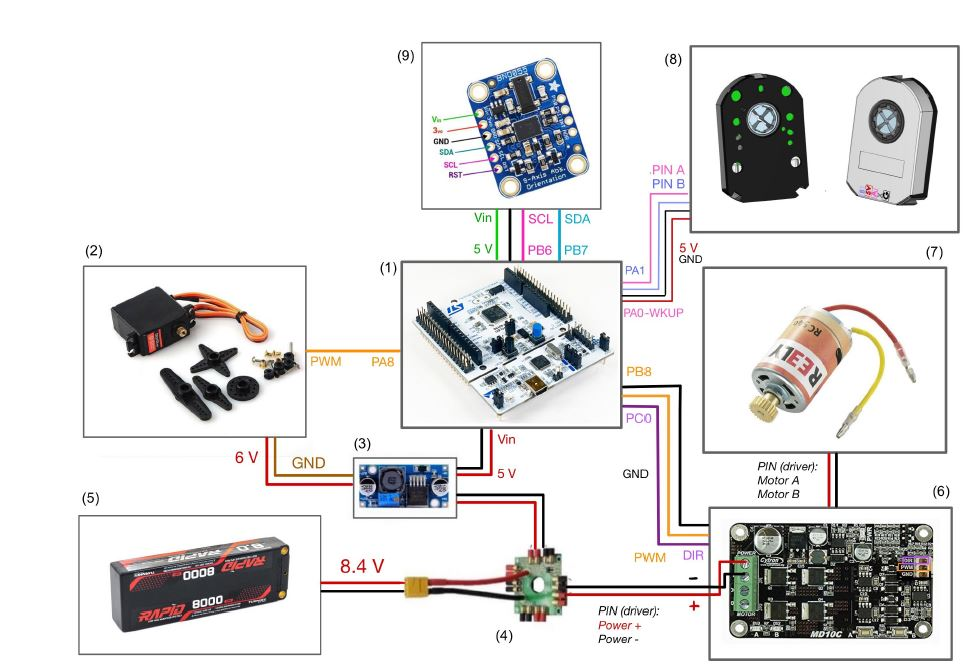
\includegraphics[width=0.8\textwidth,keepaspectratio]{figures/Schema.JPG}
% \caption{Schema dei collegamenti}
% \label{fig:schema}
% \end{figure}

\section{Integrazione ROS-Unity}

\subsection{ROS-TCP Connector}
\subsection{ROS-TCP Endpoint }
\subsection{URDF Importer}

\section{Moveit}

\section{Gazebo}

\section{Cloth di Unity}
Il sistema \textbf{Cloth di Unity} offre una soluzione basata sulla fisica per simulare tessuti e materiali flessibili all'interno di ambienti 3D. Sebbene sia stato progettato principalmente per rappresentare abbigliamento su personaggi, può essere utilizzato anche per altri scopi, come bandiere, tende o qualsiasi altro oggetto che richieda una simulazione realistica del comportamento dei tessuti\cite{ManualCloth}.
In questo progetto, il componente Cloth riveste un ruolo central,poiché il compito finale prevede che l'indumento manipolato dal robot presenti una fisica il più possibile realistica, simulando accuratamente il comportamento del tessuto. A tal fine, sono stati forniti tre file principali relativi a una maglietta: un file \textbf{OBJ}, un file \textbf{FBX} e un fil \textbf{Collada}. 
L'analisi di questi file ha permesso di ottenere informazioni utili riguardo al formato da utilizzare e alle caratteristiche della mesh per applicare efficacemente il componente Cloth.
\subsection{Compatibilità dei file con Gazebo e Unity}
Il formato \textbf{.obj} è stato testato con successo sia in Unity che in Gazebo, consentendo l'importazione corretta del modello della t-shirt in entrambi i software. Tuttavia, durante le simulazioni in Unity, l'applicazione del componente Cloth alla t-shirt ha evidenziato alcune difficoltà: il computer ha riscontrato problemi nel gestire correttamente i comandi impostati e, una volta avviata la simulazione, la t-shirt appariva deformata e non realistica, come è possibile vedere nella figura \ref{fig:cloth_error}.

\begin{figure}[h!]
    \centering
    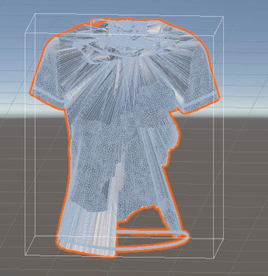
\includegraphics[width=0.4\textwidth]{images/cloth_error.PNG}
    \caption{Errore nell'applicazione del Cloth di Unity}
    \label{fig:cloth_error}
\end{figure}

Per risolvere questo problema, l'oggetto è stato importato nel software Blender, dove è stato utilizzato il modificatore Decimate per ridurre il numero di poligoni della mesh. Diminuendo il parametro "Ratio" a un valore che ha portato la mesh a circa 5000 poligoni, è stato possibile reimportare l'oggetto in Unity e applicare correttamente il componente Cloth, ottenendo una simulazione più realistica.

\begin{figure}[h!]
    \centering
    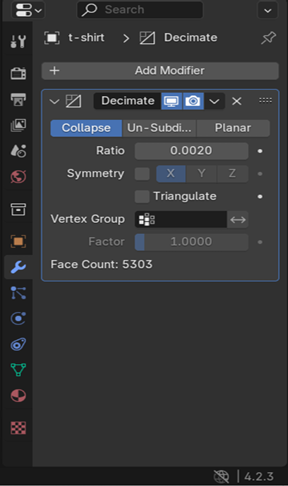
\includegraphics[width=0.3\textwidth]{images/blender_ratio.PNG}
    \caption{Modifica della Mesh nel software Blender}
    \label{fig:blender_ratio}
\end{figure}

Il formato \textbf{.fbx} non è supportato da Gazebo; tuttavia, è compatibile con Unity e può essere convertito in altri formati, come .obj o .dae (Collada), utilizzando Blender. Seguendo lo stesso procedimento adottato per il file .obj, quindi riducendo il numero di poligoni delle mesh tramite il modificatore Decimate in Blender, la simulazione in Unity è stata eseguita correttamente.

Il formato  \textbf{.dae} (Collada) è supportato da Gazebo e risulta essere ampiamente utilizzato in questo contesto. Importando i file .obj della t-shirt e della scarpa, nonché il file .fbx della t-shirt in Blender, è stato possibile esportarli nel formato .dae. Questa operazione ha permesso di caricare correttamente i vari modelli in Gazebo, facilitando la simulazione degli indumenti nel simulatore.

In sintesi, l'utilizzo combinato di Blender per l'ottimizzazione delle mesh e la conversione dei formati, insieme all'applicazione del componente Cloth in Unity, ha consentito di ottenere simulazioni più realistiche del comportamento dei tessuti, migliorando l'interazione tra il robot e gli indumenti nel contesto del progetto.

\subsection{Componente Cloth e relativo Manuale}
Tra la documentazione di Unity è possibile trovare anche quella relativa al componente Cloth e in seguito verranno riassunti i passaggi fondamentali per utilizzarlo al meglio.

Per implementare una simulazione di tessuto in Unity, è necessario aggiungere il componente Cloth a un oggetto mesh. Ecco i passaggi fondamentali:
\begin{itemize}
    \item \textbf{Preparazione della Mesh}: è importante assicurarsi che l'oggetto a cui si desidera applicare il tessuto abbia una mesh adeguata, e quindi, come visto in precedenza, anche un numero adeguato di poligoni della mesh.
    
    \item \textbf{Aggiunta del Componente}: una volta importato il file su Unity è sufficiente selezionare l'oggetto nella gerarchia di Unity e, nel pannello Inspector, cliccare su "Add Component", selezionare "Physics" e poi "Cloth" dalla lista dei componenti disponibili.

    \item \textbf{Configurazione}: Una volta aggiunto il componente, sarà possibile modificare vari parametri per ottenere una simulazione personalizzata e accurata.
\end{itemize}
\newpage
Affinchè la maglietta abbia una movimentazione guidata dalla fisica, deve chiaramente avere una parte della maglietta fissata e che quindi non è soggetta alla gravità. Questi su Unity vengono chiamati "Cloth Constraint" e quindi ""vincoli del Cloth".
Di seguito una descrizione dei passaggi per applicarli correttamente alla maglietta:
\begin{enumerate}
    \item sul component Cloth si clicca su "Edit Cloth Constraint" come possiamo vedere dalla figura \ref{fig:cloth_constraints}
    \begin{figure}[h!]
        \centering
        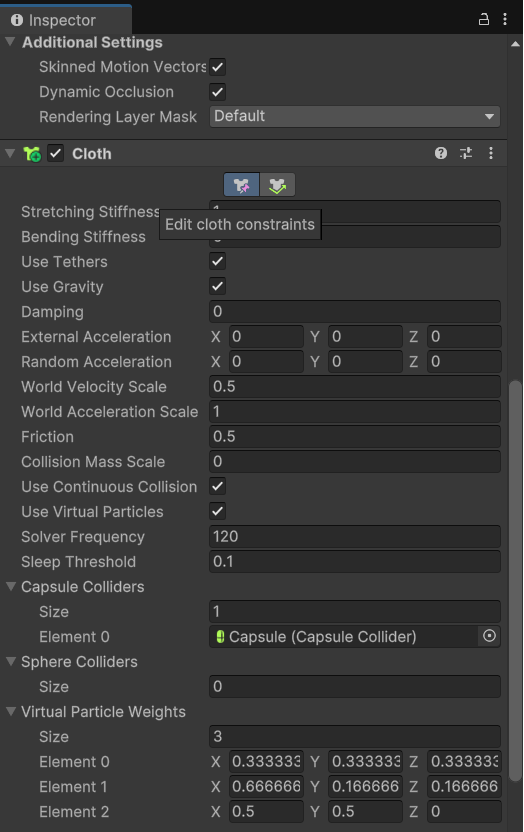
\includegraphics[width=0.3\textwidth]{images/cloth_constraints.PNG}
        \caption{Schermata Unity per l'applicazione dei vincoli}
        \label{fig:cloth_constraints}
    \end{figure}
    \item successivamente si aprirà una schermata che permetterà di selezionare (tramite "Select") oppure colorare (tramite "Paint") le parti che saranno vincolate e quindi rimarranno maggiormente rigide. E' importante specificare una distanza minima nel parametro "Max Distance", in figura \ref{fig:cloth_constraints_2} è stato assegnato il valore 0.2 ed ha permesso un buon risultato.
    \begin{figure}[h!]
        \centering
        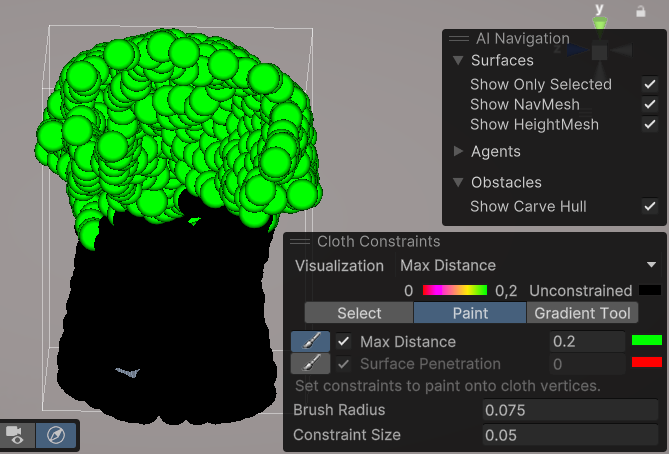
\includegraphics[width=0.5\textwidth]{images/cloth_constraints_2.PNG}
        \caption{Schermata Unity per la selezione delle parti della mesh a cui applicare i vincoli}
        \label{fig:cloth_constraints_2}
    \end{figure}
\end{enumerate}



Infine una descrizione delle principali proprietà del componente Cloth e di come sono state utilizzate nell'implementazione del tessuto realistico della maglietta:
\begin{itemize}
    \item \textbf{Stretching Stiffness}: Determina la resistenza del tessuto all'allungamento. Valori più alti rendono il tessuto meno incline a estendersi.

    \item \textbf{Bending Stiffness}: Controlla la rigidità alla flessione del tessuto. Un valore elevato riduce la capacità del tessuto di piegarsi.
    
    \item \textbf{Use Tethers}: Applica vincoli che aiutano a prevenire che le particelle mobili del tessuto si allontanino troppo da quelle fisse, riducendo l'eccessiva elasticità.
    
    \item \textbf{Use Gravity}: Indica se la gravità deve influenzare il tessuto.
    
    \item \textbf{Damping}: Coefficiente che determina quanto velocemente il movimento del tessuto si smorza nel tempo.
    
    \item \textbf{External Acceleration}: Applica un'accelerazione costante esterna al tessuto, utile per simulare effetti come il vento.
    
    \item \textbf{Random Acceleration}: Introduce un'accelerazione casuale al tessuto, aggiungendo variazioni imprevedibili nel movimento.
    
    \item \textbf{World Velocity Scale}: Determina quanto il movimento in spazio globale dell'oggetto influisce sui vertici del tessuto.
    
    \item \textbf{World Acceleration Scale}: Controlla l'influenza dell'accelerazione globale dell'oggetto sui vertici del tessuto.
    
    \item \textbf{Friction}: Imposta il coefficiente di attrito del tessuto durante le collisioni.
    
    \item \textbf{Collision Mass Scale}: Determina l'incremento di massa delle particelle durante le collisioni.
    
    \item \textbf{Use Continuous Collision}: Abilita la collisione continua per migliorare la stabilità delle interazioni.
    
    \item \textbf{Use Virtual Particles}: Aggiunge particelle virtuali per migliorare la stabilità delle collisioni.
    
    \item \textbf{Solver Frequency}: Specifica il numero di iterazioni del solver per secondo, influenzando la precisione della simulazione.
    
    \item \textbf{Sleep Threshold}: Definisce la soglia sotto la quale il tessuto entra in stato di "sonno", interrompendo la simulazione fino a nuove interazioni.
    
    \item \textbf{Capsule Colliders}: Array di collisori a capsula con cui il tessuto può interagire.
    
    \item \textbf{Sphere Colliders}: Array di coppie di collisori sferici con cui il tessuto può interagire.
\end{itemize}

\subsection{Componente Cloth e collisioni con altri materiali}
\section{Camera}

\chapter{Risultati ottenuti e discussione}
% Nell'introduzione al capitolo specificate anche la versione dell'STM32CubeIDE e dell'STM32CubeMX che avete usato (se avete cambiato versione nel corso del progetto mettete l'ultima, quella su cui è sviluppato il codice che consegnate).

% \section{Diagramma di flusso}
% Inserire un diagramma di flusso analogo a quello in Figura \ref{fig:diagramma} che spiega il funzionamento generale del codice sviluppato. Inserire anche una descrizione testuale del funzionamento.

% \begin{figure}[H]
% \centering
% 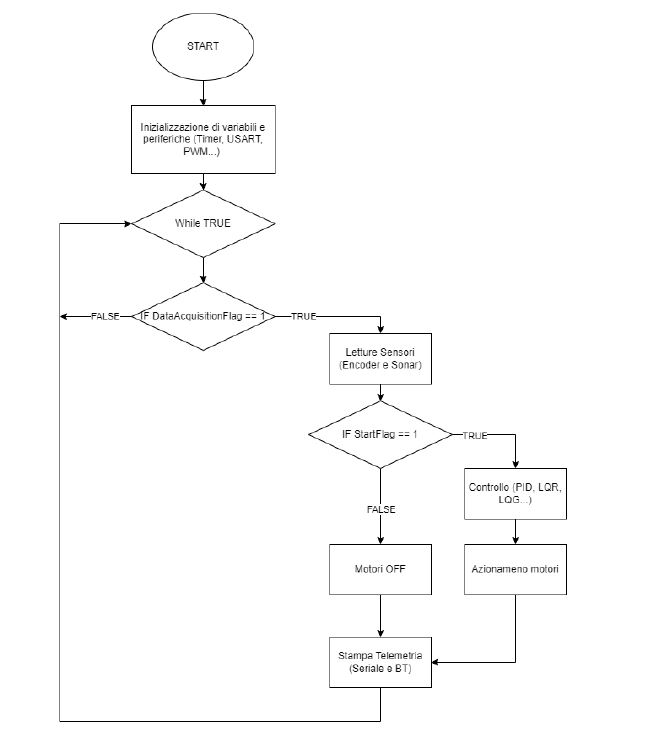
\includegraphics[width=0.8\textwidth,keepaspectratio]{figures/diagramma.JPG}
% \caption{Diagramma di flusso del codice sviluppato}
% \label{fig:diagramma}
% \end{figure}

% \section{Gestione singoli componenti}
% Dedicare un pagagrafo ad ogni componente in cui viene spiegato il codice che lo gestisce. Inserite prima una descrizione generale di come si gestisce un componente di quel tipo (aiutandovi con schemi o altro). Poi le configurazioni che sono state fatte sul .ioc per poterlo utilizzare (quale periferiche sono state abilitate, come sono state configurate.. mettete degli screen del .ioc). Infine inserite e spiegate le parti di codice che lo gestiscono.\\
% \newline
% \textcolor{red}{NOTA per il codice}: per rendere il codice modulare e riutilizzabile è buona prassi non caricare troppo il main ma creare una libreria per ogni componente. Quindi il componente1 avrà un header file "componente1.h" e un source file "componente1.c", nel source file sono implementate le funzioni che gestiscono il componente, nell'header file ci sono i prototipi di tali funzioni in modo che esse possano essere usate nel main includendolo.\\
% \newline
% \textcolor{red}{NOTA per il codice}: non inserire mai nel codice dei parametri numerici senza contesto ma renderli delle costanti definite (usando la direttiva \%define). Se sono delle costanti relative ad uno specifico componente vanno inserite nel relativo header file.\\
% \newline
% \textcolor{red}{NOTA per il codice}: per inserire il codice, anziché utilizzare screenshot utilizzate i seguenti comandi.\\
% Per codice scritto in latex (con linguaggio Python):
% \begin{lstlisting}[language=Python, caption="Codice in Python"]
% import numpy as np
    
% def incmatrix(genl1,genl2):
%     m = len(genl1) # The length of the first array
%     n = len(genl2) # The length of the second array
%     sum = 0
    
%     # Compute 
%     for i in range(0,n):
%         for j in range(0, m):
%             sum += genl1[n]*genl2[m]

%     # Print
%     print("The sum is %2d" %(sum))   
    
%     return M
% \end{lstlisting}
% Per codice richiamato da file (con linguaggio C):

% \lstinputlisting[language=Cpp, firstline=4, lastline=8, caption="Codice in C"]{codefiles/example_code.cpp}

% Funziona anche per codice MATLAB:
% \begin{lstlisting}[language=MATLABc, caption="Codice in MATLAB"]
% %% PREPARE WORKSPACE
% close all
% clearvars
% clc

% %% OPERATIONS
% sayhello;

% %% FUNCTIONS
% function sayhello
%     fprintf("Hello world!");
% end

% \end{lstlisting}


% \subsection{Gestione componente1}

% \subsection{Gestione componente2}

% \section{Funzionamento complessivo}
% Dopo aver spiegato il codice che gestisce i singoli componenti, inserire e commentare le porzioni di codice relative al funzionamento complessivo del programma.

\chapter{Conclusioni e prospettive future}
% Dedicate un capitolo a tutti i test effettuati con relativi risultati, includete sia i test finali relativi al funzionamento complessivo, sia i test delle singole parti (se significativi). \\
% Descrivete in dettaglio le condizioni in cui sono stati svolti i test in modo che siano ripetibili. Durante i test fate dei video e acquisite i dati (es usando la funzione di log di Putty), per i test più rilevanti è opportuno consegnare anche questo materiale per documentare i test effettuati. Nella relazione riportate i risultati con dei grafici come quello in Figura \ref{fig:grafico} (inserite sempre nei grafici le label sugli assi con grandezza e relativa unità di misura). Commentate in modo critico i risultati ottenuti, evidenziando sia quelli positivi sia quelli negativi. 

% \begin{figure}[H]
% \centering
% 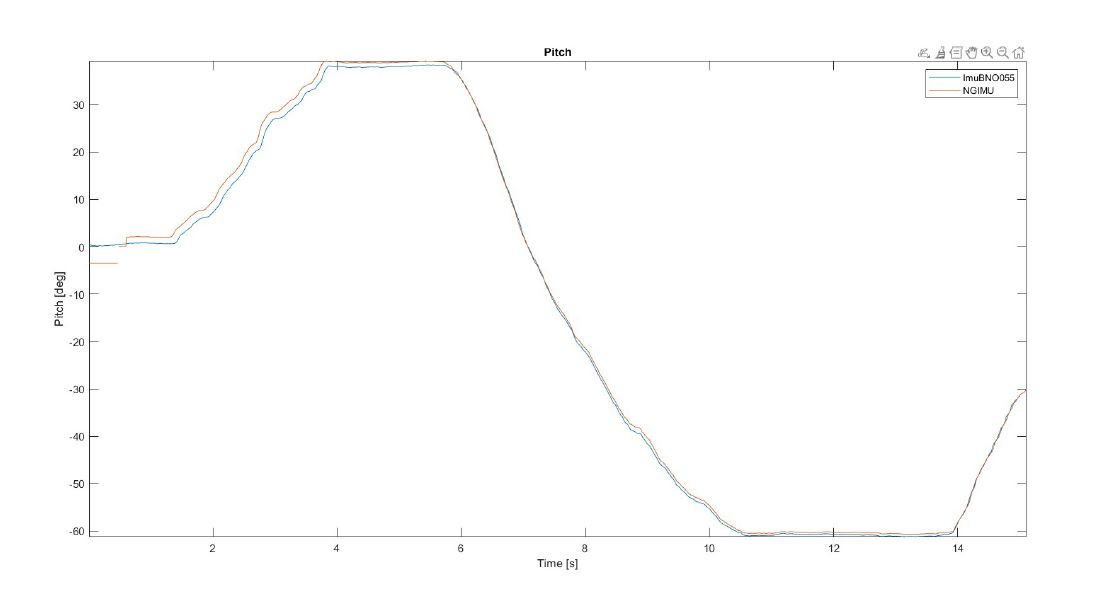
\includegraphics[width=0.8\textwidth,keepaspectratio]{figures/grafico.JPG}
% \caption{Esempio di grafico}
% \label{fig:grafico}
% \end{figure}
% \section{Test1}
% Per ogni test riportate: cosa state testando, in che condizioni si è svolto il test, riferimenti a video/file di log che consegnate insieme a relazione e codice, grafici dei risultati, commento dei risultati.

% \section{Test2}

% \newpage
% \addcontentsline{toc}{chapter}{Conclusioni e sviluppi futuri}
% \section*{Conclusioni e sviluppi futuri}
% Riassumere brevemente il lavoro svolto rispetto al task assegnato, evidenziando quali risultati sono stati raggiunti e quali no. Se ci sono aspetti del task non completati spiegare quali sono stati i problemi riscontrati in merito.\\
% Inserire considerazioni personali su possibili sviluppi futuri dell'attività svolta (idee per migliorarla che non avete avuto modo di sperimentare, aspetti che suggerite di approfondire, problemi da risolvere..).

\addcontentsline{toc}{chapter}{Appendici}
\appendix
\chapter{Appendice1}
Se necessario ricorrete alle appendici per spiegare le parti "di contorno" dell'attività svolta e/o ciò che non riuscite ad inserire nello schema generale dei capitoli della relazione (es acquisizione dei dati con Matlab).


\bibliographystyle{ieeetr}
\bibliography{bibl} 
\end{document}
